% Created by tikzDevice version 0.12.6 on 2024-03-12 19:53:24
% !TEX encoding = UTF-8 Unicode
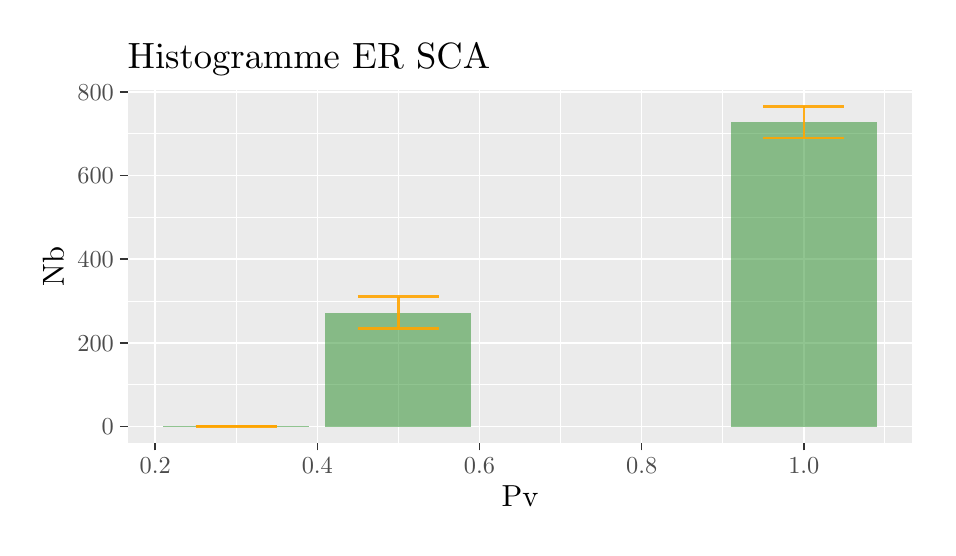
\begin{tikzpicture}[x=1pt,y=1pt]
\definecolor{fillColor}{RGB}{255,255,255}
\path[use as bounding box,fill=fillColor,fill opacity=0.00] (0,0) rectangle (325.21,180.67);
\begin{scope}
\path[clip] (  0.00,  0.00) rectangle (325.21,180.67);
\definecolor{drawColor}{RGB}{255,255,255}
\definecolor{fillColor}{RGB}{255,255,255}

\path[draw=drawColor,line width= 0.6pt,line join=round,line cap=round,fill=fillColor] (  0.00,  0.00) rectangle (325.21,180.68);
\end{scope}
\begin{scope}
\path[clip] ( 36.11, 30.69) rectangle (319.71,158.02);
\definecolor{fillColor}{gray}{0.92}

\path[fill=fillColor] ( 36.11, 30.69) rectangle (319.71,158.02);
\definecolor{drawColor}{RGB}{255,255,255}

\path[draw=drawColor,line width= 0.3pt,line join=round] ( 36.11, 51.66) --
	(319.71, 51.66);

\path[draw=drawColor,line width= 0.3pt,line join=round] ( 36.11, 81.89) --
	(319.71, 81.89);

\path[draw=drawColor,line width= 0.3pt,line join=round] ( 36.11,112.11) --
	(319.71,112.11);

\path[draw=drawColor,line width= 0.3pt,line join=round] ( 36.11,142.34) --
	(319.71,142.34);

\path[draw=drawColor,line width= 0.3pt,line join=round] ( 75.37, 30.69) --
	( 75.37,158.02);

\path[draw=drawColor,line width= 0.3pt,line join=round] (133.97, 30.69) --
	(133.97,158.02);

\path[draw=drawColor,line width= 0.3pt,line join=round] (192.56, 30.69) --
	(192.56,158.02);

\path[draw=drawColor,line width= 0.3pt,line join=round] (251.16, 30.69) --
	(251.16,158.02);

\path[draw=drawColor,line width= 0.3pt,line join=round] (309.75, 30.69) --
	(309.75,158.02);

\path[draw=drawColor,line width= 0.6pt,line join=round] ( 36.11, 36.55) --
	(319.71, 36.55);

\path[draw=drawColor,line width= 0.6pt,line join=round] ( 36.11, 66.77) --
	(319.71, 66.77);

\path[draw=drawColor,line width= 0.6pt,line join=round] ( 36.11, 97.00) --
	(319.71, 97.00);

\path[draw=drawColor,line width= 0.6pt,line join=round] ( 36.11,127.22) --
	(319.71,127.22);

\path[draw=drawColor,line width= 0.6pt,line join=round] ( 36.11,157.45) --
	(319.71,157.45);

\path[draw=drawColor,line width= 0.6pt,line join=round] ( 46.07, 30.69) --
	( 46.07,158.02);

\path[draw=drawColor,line width= 0.6pt,line join=round] (104.67, 30.69) --
	(104.67,158.02);

\path[draw=drawColor,line width= 0.6pt,line join=round] (163.26, 30.69) --
	(163.26,158.02);

\path[draw=drawColor,line width= 0.6pt,line join=round] (221.86, 30.69) --
	(221.86,158.02);

\path[draw=drawColor,line width= 0.6pt,line join=round] (280.46, 30.69) --
	(280.46,158.02);
\definecolor{fillColor}{RGB}{34,139,34}

\path[fill=fillColor,fill opacity=0.50] ( 49.00, 36.55) rectangle (101.74, 36.57);

\path[fill=fillColor,fill opacity=0.50] (107.60, 36.55) rectangle (160.33, 77.73);

\path[fill=fillColor,fill opacity=0.50] (254.09, 36.55) rectangle (306.82,146.47);
\definecolor{drawColor}{RGB}{255,165,0}

\path[draw=drawColor,draw opacity=0.90,line width= 0.9pt,line join=round] ( 60.72, 36.67) --
	( 90.02, 36.67);

\path[draw=drawColor,draw opacity=0.90,line width= 0.9pt,line join=round] ( 75.37, 36.67) --
	( 75.37, 36.47);

\path[draw=drawColor,draw opacity=0.90,line width= 0.9pt,line join=round] ( 60.72, 36.47) --
	( 90.02, 36.47);

\path[draw=drawColor,draw opacity=0.90,line width= 0.9pt,line join=round] (119.32, 83.49) --
	(148.62, 83.49);

\path[draw=drawColor,draw opacity=0.90,line width= 0.9pt,line join=round] (133.97, 83.49) --
	(133.97, 71.97);

\path[draw=drawColor,draw opacity=0.90,line width= 0.9pt,line join=round] (119.32, 71.97) --
	(148.62, 71.97);

\path[draw=drawColor,draw opacity=0.90,line width= 0.9pt,line join=round] (265.81,152.23) --
	(295.10,152.23);

\path[draw=drawColor,draw opacity=0.90,line width= 0.9pt,line join=round] (280.46,152.23) --
	(280.46,140.71);

\path[draw=drawColor,draw opacity=0.90,line width= 0.9pt,line join=round] (265.81,140.71) --
	(295.10,140.71);
\end{scope}
\begin{scope}
\path[clip] (  0.00,  0.00) rectangle (325.21,180.67);
\definecolor{drawColor}{gray}{0.30}

\node[text=drawColor,anchor=base east,inner sep=0pt, outer sep=0pt, scale=  0.88] at ( 31.16, 33.52) {0};

\node[text=drawColor,anchor=base east,inner sep=0pt, outer sep=0pt, scale=  0.88] at ( 31.16, 63.74) {200};

\node[text=drawColor,anchor=base east,inner sep=0pt, outer sep=0pt, scale=  0.88] at ( 31.16, 93.97) {400};

\node[text=drawColor,anchor=base east,inner sep=0pt, outer sep=0pt, scale=  0.88] at ( 31.16,124.19) {600};

\node[text=drawColor,anchor=base east,inner sep=0pt, outer sep=0pt, scale=  0.88] at ( 31.16,154.42) {800};
\end{scope}
\begin{scope}
\path[clip] (  0.00,  0.00) rectangle (325.21,180.67);
\definecolor{drawColor}{gray}{0.20}

\path[draw=drawColor,line width= 0.6pt,line join=round] ( 33.36, 36.55) --
	( 36.11, 36.55);

\path[draw=drawColor,line width= 0.6pt,line join=round] ( 33.36, 66.77) --
	( 36.11, 66.77);

\path[draw=drawColor,line width= 0.6pt,line join=round] ( 33.36, 97.00) --
	( 36.11, 97.00);

\path[draw=drawColor,line width= 0.6pt,line join=round] ( 33.36,127.22) --
	( 36.11,127.22);

\path[draw=drawColor,line width= 0.6pt,line join=round] ( 33.36,157.45) --
	( 36.11,157.45);
\end{scope}
\begin{scope}
\path[clip] (  0.00,  0.00) rectangle (325.21,180.67);
\definecolor{drawColor}{gray}{0.20}

\path[draw=drawColor,line width= 0.6pt,line join=round] ( 46.07, 27.94) --
	( 46.07, 30.69);

\path[draw=drawColor,line width= 0.6pt,line join=round] (104.67, 27.94) --
	(104.67, 30.69);

\path[draw=drawColor,line width= 0.6pt,line join=round] (163.26, 27.94) --
	(163.26, 30.69);

\path[draw=drawColor,line width= 0.6pt,line join=round] (221.86, 27.94) --
	(221.86, 30.69);

\path[draw=drawColor,line width= 0.6pt,line join=round] (280.46, 27.94) --
	(280.46, 30.69);
\end{scope}
\begin{scope}
\path[clip] (  0.00,  0.00) rectangle (325.21,180.67);
\definecolor{drawColor}{gray}{0.30}

\node[text=drawColor,anchor=base,inner sep=0pt, outer sep=0pt, scale=  0.88] at ( 46.07, 19.68) {0.2};

\node[text=drawColor,anchor=base,inner sep=0pt, outer sep=0pt, scale=  0.88] at (104.67, 19.68) {0.4};

\node[text=drawColor,anchor=base,inner sep=0pt, outer sep=0pt, scale=  0.88] at (163.26, 19.68) {0.6};

\node[text=drawColor,anchor=base,inner sep=0pt, outer sep=0pt, scale=  0.88] at (221.86, 19.68) {0.8};

\node[text=drawColor,anchor=base,inner sep=0pt, outer sep=0pt, scale=  0.88] at (280.46, 19.68) {1.0};
\end{scope}
\begin{scope}
\path[clip] (  0.00,  0.00) rectangle (325.21,180.67);
\definecolor{drawColor}{RGB}{0,0,0}

\node[text=drawColor,anchor=base,inner sep=0pt, outer sep=0pt, scale=  1.10] at (177.91,  7.64) {Pv};
\end{scope}
\begin{scope}
\path[clip] (  0.00,  0.00) rectangle (325.21,180.67);
\definecolor{drawColor}{RGB}{0,0,0}

\node[text=drawColor,rotate= 90.00,anchor=base,inner sep=0pt, outer sep=0pt, scale=  1.10] at ( 13.08, 94.35) {Nb};
\end{scope}
\begin{scope}
\path[clip] (  0.00,  0.00) rectangle (325.21,180.67);
\definecolor{drawColor}{RGB}{0,0,0}

\node[text=drawColor,anchor=base west,inner sep=0pt, outer sep=0pt, scale=  1.32] at ( 36.11,166.08) {Histogramme ER SCA};
\end{scope}
\end{tikzpicture}
